\documentclass[12pt]{ULrapport}
\usepackage[utf8]{inputenc}
\usepackage[french]{babel}
\usepackage{float}
\restylefloat{table}
\usepackage{hhline}
\usepackage{pdfpages}
\usepackage{hyperref}
\usepackage{lscape}
\usepackage{pdflscape}




% Title Page
\title{Design 3}
\author{Name 1, Name 2, Rémi Mercier, Name 4}



\TitreProjet{Pirates des Caraïbes}
\TitreRapport{Rapport de développement}
\Destinataire{Dominique Grenier, Philippe Giguère, Denis Laurendeau}
\NumeroEquipe{4}
%\NomEquipe{Équipe 1}
\TableauMembres{%
	111\,076\,721  & Mercier, Rémi     & \\\hline
	111\,076\,680  & Bilodeau, Dominic     & \\\hline
	111\,073\,278  & Béland, Camille     & \\\hline
	111\,040\,716  & Arel, David     & \\\hline
	111\,096\,321  & B. Bolduc, Adam     & \\\hline
	111\,075\,609  & Lévesque, Mathieu    & \\\hline
	908\,188\,831  & Papillon, Maxime  & \\\hline
	907\,152\,804  & Jean-Christophe Martin-Morin & \\\hline
}
\DateRemise{17 avril 2016}
% Contenu de l'historique des versions
\HistoriqueVersions{%										% version & date & description \\\hline
	   1.0  & 31 janvier 2016 & - Livrable 1 \\\hline
	   2.0  & 28 février 2016 & - Livrable 2 \\\hline
	   3.0  & 3 avril 2016 & - Livrable 3 \\\hline
	   4.0  & 17 avril 2016 & - Livrable 4 \\\hline
}

\begin{document}
\maketitle
\listoffigures

%!TEX encoding = IsoLatin

\chapter{Introduction}
Le pr�sent rapport pr�sente le livrable 1 du projet Pirate des cara�bes pour le cours de Design III. Le projet consiste � d�velopper un robot autonome capable de rep�rer des pi�ces ferromagn�tiques repr�sentant des tr�sors, de les ramasser et d'aller les d�poser sur l'�le sp�cifi�e au d�but du d�fi. Plusieurs disciplines du g�nie sont requises afin d'accomplir la t�che, il est donc important de bien identifier les requis et d'avoir une id�e structur�e du probl�me d�s le d�part. Ce rapport pr�sente donc le r�sultat de la d�composition technique du probl�me. Il comporte la d�finition des proprit�s fonctionnelles, la description des cas d'utilisation, les diagrammes d'architecture logicielle, ainsi que la description des exp�rimentations r�alis�es par l'�quipe jusqu'� maintenant.

\chapter{Description des propriétés fonctionnelles}
La Description des propriétés fonctionnelles (DPF), se retrouvant à l'annexe \ref{annexe_dpf}, permet de visualiser les exigences du client ainsi que de les associer aux fonctionnalités du produit.

\section{Détails des exigences}

\paragraph{10 minutes pour effectuer toutes les tâches:}
Le temps pour effectuer toutes les étapes d'un cycle de jeu est de 10 minutes. Le chronomètre part au moment où le signal de départ est donné au robot.
Plusieurs cycles de jeu peuvent être effectués durant les 10 minutes prescrits.

\paragraph{Recharge de l'électro-aimant par induction:}
Le condensateur qui va contenir la charge que l'électro-aimant va utiliser doit être rechargé par induction à la station de recharge.

\paragraph{Alimenter l'électro-aimant avec un condensateur:}
L'électro-aimant doit absolument être alimenté par un condensateur et non par un autre type d'alimentation.

\paragraph{Soulever les trésor avec l'électro-aimant:}
Le trésor doit être soulevé à l'aide d'un électro-aimant alimenté par un condensateur. La charge doit être suffisante afin de transporter le trésor jusqu'à l'île prescrite.

\paragraph{Le robot ne peut toucher aux bords ou aux îles:}
Dans tous ses déplacements, le robot ne peut toucher aux murs de la zone de jeu. Une seule offense est tolérée.

\paragraph{Afficher la trajectoire planifié du robot:}
Tous les déplacements du robot doivent être annoncés à l'avance.

\paragraph{Afficher la couleur ou la forme de l'île prescrite:} Une fois la requête serveur faite, le système doit afficher sur la station de base la couleur et la forme de l'île identifiée.

\paragraph{Afficher la position du robot:}
La position estimée du robot doit être affichée sur l'interface utilisateur. Cette position a une incertitude de 15 cm par rapport à la position réelle.

\paragraph{Afficher le voltage au bornes du condensateur:}
Le voltage du condensateur servant à alimenter l'électro-aimant doit être affiché sur l'interface utilisateur en tout temps.

\paragraph{Le code Manchester doit être capter sans-fil:}
La méthode d'acquisition du code Manchester doit être sans-fil, le spectre utilisé n'est pas important.

\paragraph{Le décodage ne doit pas être effectué dans la station de recharge:}
Il faut attendre que le condensateur soit plein avant de décoder le code Manchester.

\paragraph{Une seule requête serveur par cycle de jeu:}
Après l'aquisition du code Manchester, une seule requête serveur peut être faite par cycle de jeu.

\paragraph{Le trésor doit être déposé sur la bonne île:}
Le trésor doit être déposé sur l'île identifiée à l'aide du code Manchester et de la requête serveur.

\paragraph{Le robot doit être alimenté par batterie:}
Tous les systèmes montés sur le robot doivent être alimentés par un système de batterie embarqué sur le robot.

\paragraph{Toutes les alimentations doivent être protégées par fusible et/ou interrupteur:}
Afin de protéger tout l'équipement du robot, toutes les alimentation se doivent d'être protégées au minimum par un fusible ou un interrupteur.

\paragraph{Autonomie complète du robot:}
Durant tout le cycle de jeu, le robot doit être entièrement autonome dans ses déplacements et actions. Des touchettes sont autorisées avec pénalités.

\paragraph{Rafraichissement minimal de l'interface utilisateur de 0.2 Hz:}
L'interface utilisateur affichant par exemple la position du robot, les trajets planifiés ainsi que le voltage du condensateur doit être rafraichit au minimum toutes les 5 secondes.

\paragraph{Budget de 300\$ :}
En dehors du matériel fourni, l'ensemble du matériel acheté servant au robot doit coûter au maximum 300\$.

\paragraph{Apparence professionnelle:}
L'ensemble des circuits doivent être montés sur circuits imprimés. Les breadboards ne sont pas permis.

\section{Détail des fonctionnalités}

\subsection{Détecter les éléments du jeu}

\paragraph{Détecter la position et l'angle du robot:}
Le robot est en mesure de se situer dans son environnement à l'aide des différents capteurs à sa disposition.

\paragraph{Détecter les îles, leurs formes, tailles et couleurs:}
Le robot détecte les îles placées de façon aléatoire. Il identifie leur dimension, leur couleur et leur forme.

\paragraph{Détecter les trésors:}
Le robot est en mesure de détecter les trésors dans l'environnement.

\paragraph{Détecter la station de recharge:}
Le robot peut identifier la station de recharge en début de cycle de jeu.

\paragraph{Détecter les limites de la zone de jeu:}
Le robot détecte lors de ses déplacement les limites de la zone de jeu afin de ne jamais entrer en contact avec elles.

\subsection{Acquérir et décoder un code Manchester}

\paragraph{Acquérir le code Manchester sans-fil:}
Le robot peut acquérir un code Manchester à l'aide d'un protocole HF.

\paragraph{Décoder le code Manchester:}
Le robot est en mesure de décoder le code Manchester afin d'obtenir le caractère ASCII correspondant.

\paragraph{Faire une requête serveur:}
Le robot peut effectuer une requête GET ayant comme paramètre le code reçu par le signal HF.

\subsection{Trouver et manipuler un trésor}

\paragraph{Charger l'électro-aimant à la station de recharge sans-fil:}
Le robot a un dispositif permettant de charger un condensateur par induction afin d'offrir de la puissance à l'électro-aimant.

\paragraph{Choisir un trésor en fonction de sa position:}
Avec ses capteurs, le robot est en mesure de choisir un des trésor sur la zone de jeu en fonction de sa position.

\paragraph{Soulever et déposer un trésor à l'aide d'un électro-aimant:}
Avec son électro-aimant, le robot est en mesure de soulever et de déposer un trésor.

\subsection{Choisir automatiquement la prochaine action:}
Durant tout le cycle de jeu, le robot est en mesure de décider de la prochaine action. Cela comprend entre autres les déplacements, les rotations, le mouvement de la caméra embarquée
et la requête serveur pour le code Manchester.

\subsection{Alimenter le système}

\paragraph{Protéger les différents circuits:}
Toutes les alimentation sont protégées avec des fusibles ou des interrupteurs.

\paragraph{Fournir l'alimentation appropriée à chaque composante:}
Chaque composante a des besoins différents en alimentation. Le robot possède donc une alimentation pour les moteur, l'ordinateur embarqué, la caméra embarquée, le micro-contrôleur, le pololu et l'électro-aimant.

\subsection{Déplacer le robot}

\paragraph{Déplacer le robot en ligne droite:}
Avec ses 4 roues, le robot est en mesure de se déplacer dans toutes les directions dans les axes X et Y.

\paragraph{Effectuer une rotation du robot sur lui même:}
Le robot peut tourner sur lui-même à gauche ou à droite.

\paragraph{Asservir les déplacements en position et en vitesse:}
Les 4 roues sont asservies en vitesse de façon à garder une vitesse constante correspondant à la commande.

\paragraph{Déterminer un trajet pour se rendre d'un point A à un point B:}
Pour un objectif avec une position donnée, le robot peut déterminer une série de mouvement à faire pour s'y rendre.

\subsection{Afficher l'état du jeu}

\paragraph{Afficher le voltage du condensateur:}
Le robot envoie à la station de base le voltage du condensateur qui l'affiche en temps réel.

\paragraph{Afficher la carte virtuelle du jeu avec tous ses éléments:}
La station de base affiche une carte correspondant à la zone de jeu et ses éléments, incluant la position estimée du robot.

\paragraph{Afficher les déplacements planifiés du robot sur la carte:}
Les déplacements calculé par le robot sont affichés sur la carte à la station de base.

\subsection{Respecter apparences}
Aucun breadboard n'est utilisé, tous les circuits sont fait sur PCB.

\subsection{Respecter le budget}
Toutes les composantes du robot respecte le budget total de 300\$.


\begin{landscape}
  \begin{center}
    \begin{figure}[h]
      \label{annexe_dpf}
      \centering
      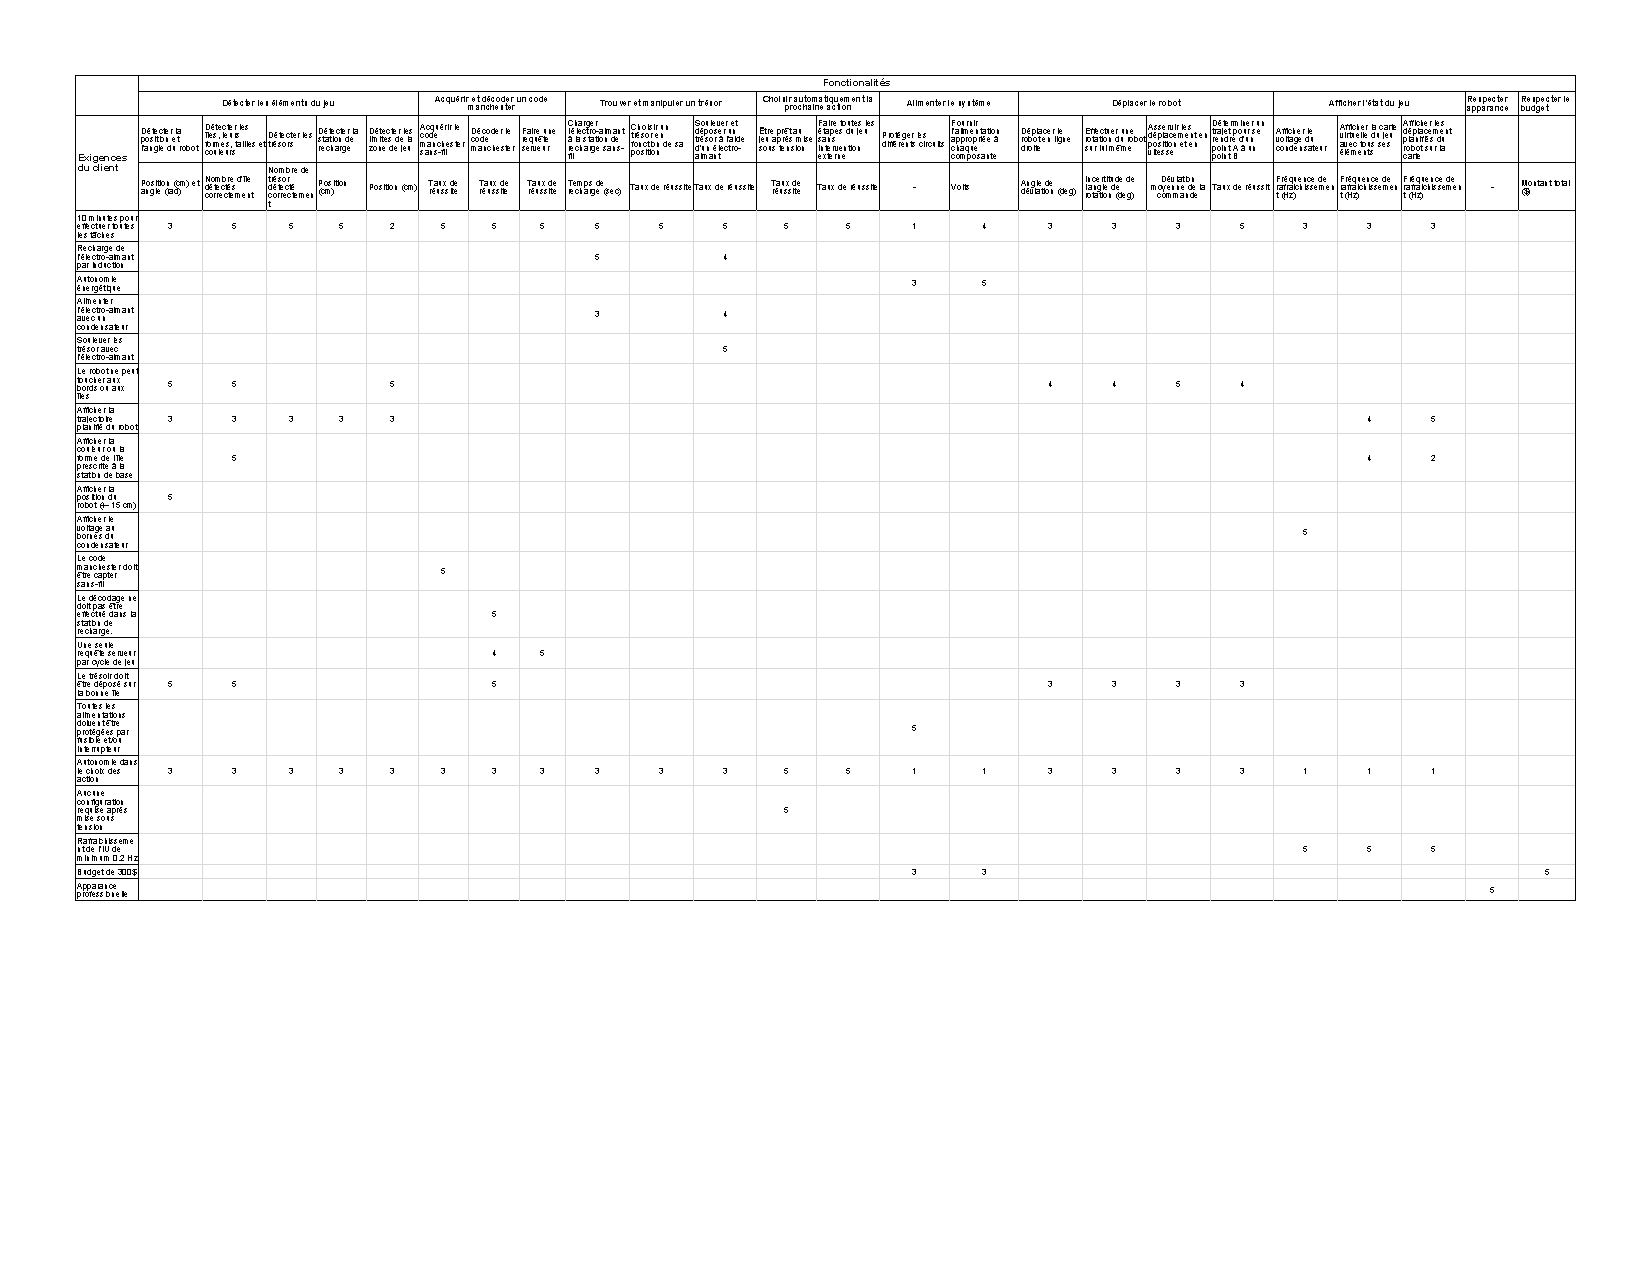
\includegraphics[scale=0.85]{resources/dpf.pdf}
      \caption{Description des propriétés fonctionnelles}
    \end{figure}
  \end{center}
\end{landscape}
\chapter{Matrice de vérification des performances}

La matrice de vérification des performances permet de visualiser les tests effectués sur le robot. Ces tests permettent de s'assurer que toutes les fonctionnalités cités par le DPF sont présentes dans le robot. Pour chaque sous-fonctionnalité, on y retrouve un ou plusieurs paramètres critiques associés ainsi que les tests effectués et les résultats obtenus.

\begin{figure}[h]
  \centering
  \caption{Matrice de vérification des performances}
  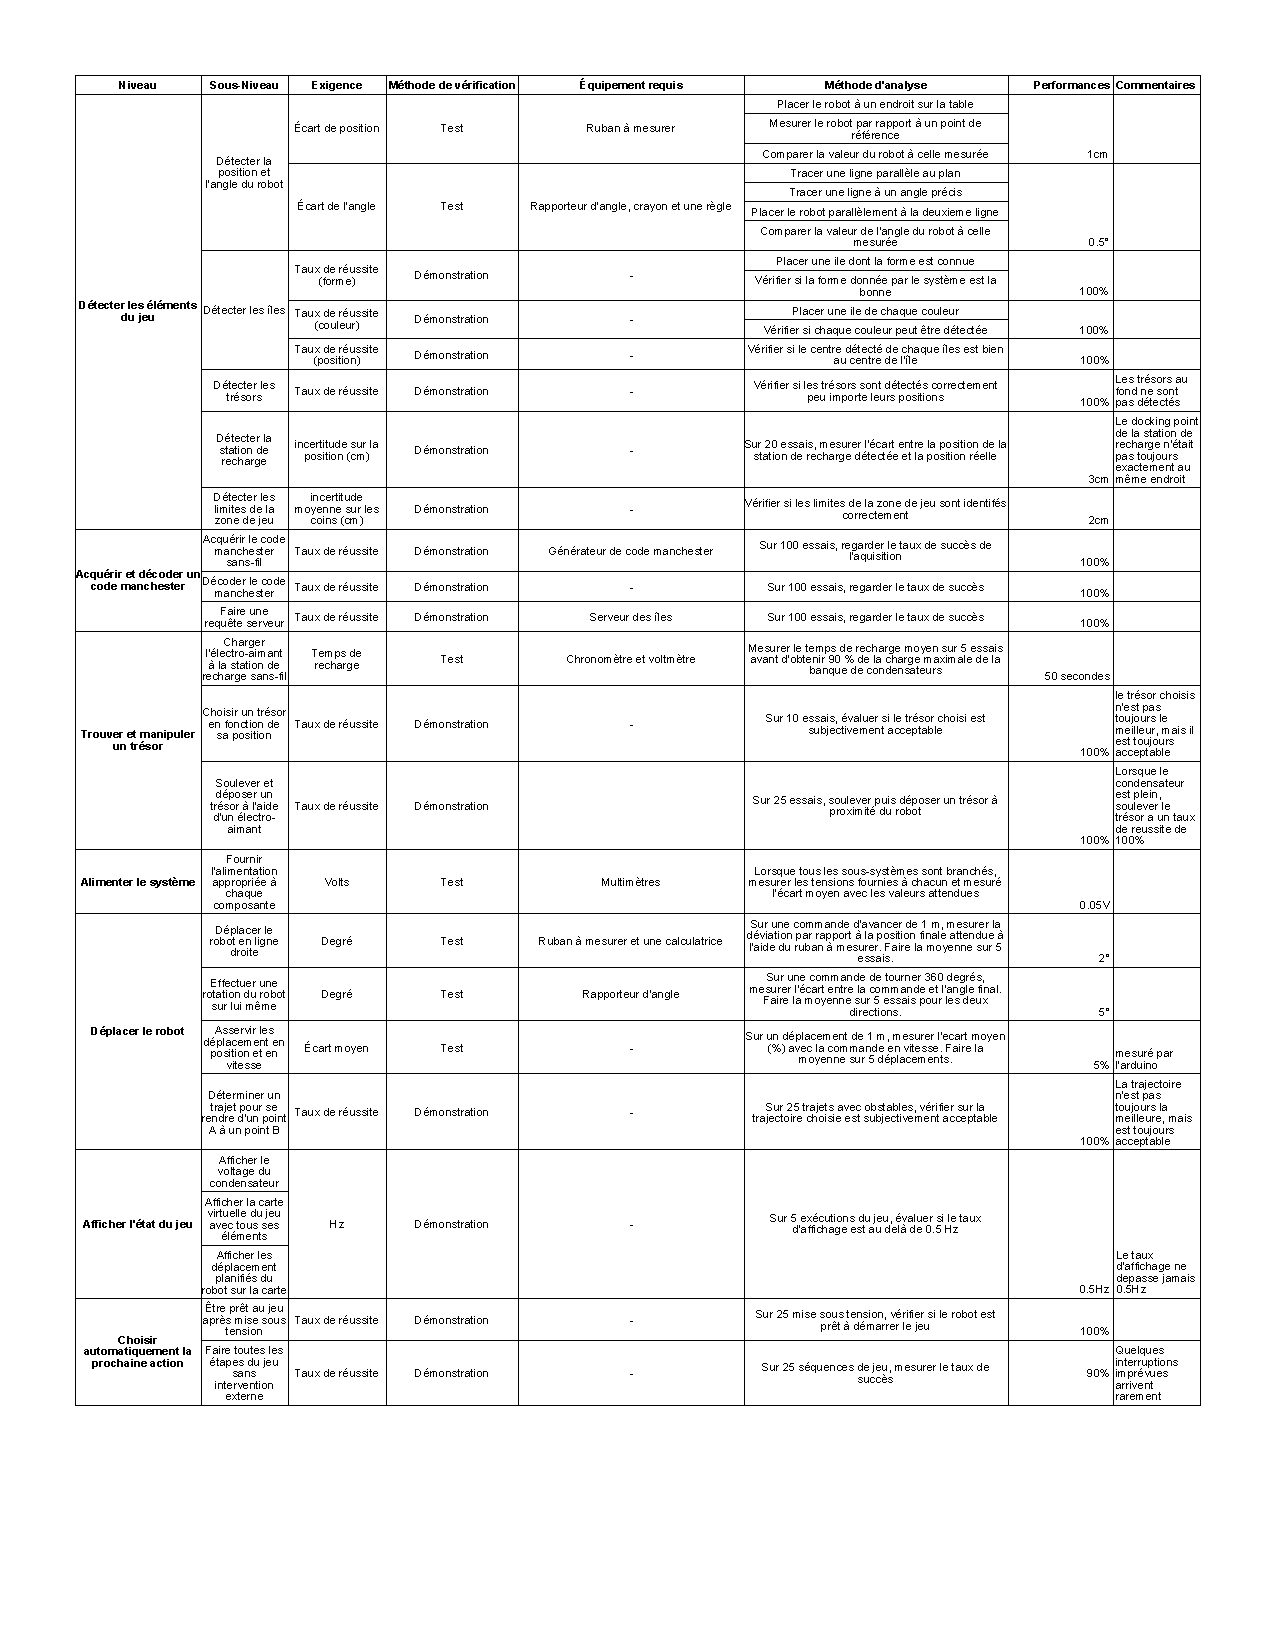
\includegraphics[scale=0.85]{resources/verification.pdf}
\end{figure}

\chapter{Vision numérique}

\section{Algorithmes}

Afin de détecter les différents éléments nécessaires au projet, différentes stratégies de traitement d'images sont utilisées dans OpenCV. Les principaux algorithmes utilisés seront décrient dans les sous-sections suivantes. Ensuite, pour chaque élément différent à détecter, la stratégie exacte utilisée avec la séquence de filtres sera expliquée.

\subsection{Gaussian Blur}

Le filtre Gaussien est un filtre moyenneur qui suit les propriétés d'une courbe de distribution gaussienne. Ses paramètres sont la déviation normale en X, en Y et la taille du kernel. Ces paramètres vont former la courbe Gausienne et donc donner le "poids" relatif de chaque pixel sur ses voisins. Plus on augmente la taille du kernel et la déviation en X ou en Y, plus on obtient une image "flou". Ce filtre permet d'enlever le bruit dans l'image et de l'uniformiser, ce qui va simplifier les traitements subséquents. Cependant, un trop grand "flou" entraîne la perte de détail et n'est donc pas souhaitable pour la détection de petits éléments.

\subsection{Color Range (inRange)}

La fonction inRange() d'OpenCV permet de transformer une image à 3 dimensions de couleurs 8 bits en une image à une seule dimension de couleur binaire, soit blanc ou noir. On y définit une gamme de couleur où tous les pixels s'y trouvant deviendront blanc. Tous ceux ne s'y trouvant pas devienent noir. Cette fonction permet donc de détecter des éléments avec un éventail de couleurs spécifiques, ce qui s'avère être une stratégie simple et efficace afin de trouver des éléments de couleur. Cependant, il est important de mettre le filtre plus large que nécessaire, particulièrement dans le traitement d'image en temps réel avec une caméra puisque des changements de lumière ou de balance des blancs suffisent à rendre un filtre trop précis totalement inutile. Selon nos expériences, il est plus facile de faire les traitements subséquents sur un filtre de couleur trop large que pas assez. Par exemple, les grandes surfaces en bois de la table sont détectéspar le filtre jaune. Puisqu'elles font de très gros contours, il est facile de les éliminer en fonction de leur aire par la suite.


\subsection{Erode et Dilate}

Les fonctions erode() et dilate() utilisées conjointement permettent d'enlever le bruit et les petites imperfections sur les contours des images binaires. La fonction erode(), comme son nom l'indique, érodent les contours sur l'image. Sur les très petits contours, erode() avec suffisamment d'itérations permet de les faire disparaitre. Sur les contours qui n'ont pas disparu en raison de leur plus grande taille, il suffit alors de faire l'opération inverse, un dilate() avec le même nombre d'itérations, afin de retrouver la taille originale du contour. Ces deux fonctions permettent par exemple d'enlever le bruit restant après un inRange() afin de garder seulement les plus grosses forment bien définies.

\subsection{Contours}

La fonction findContours() permet d'identifier une série de point formant un contour, idéalement à partir d'une image binaire comme celle formée par la fonction inRange(). Les contours trouvés correspondent à une région formant une aire fermée dans l'image binaire. Les contours peuvent être approximé afin de limiter la quantité de points trouvés et donc de limiter l'utilisation de ressources.

\subsection{Traitement sur les contours}

Un coutour correspond à une série de point formant une aire fermé. Différent traitement peuvent être fait afin de filtrer les contours indésirables. Par exemple, les fonction arcLenght() et contourArea() permettent d'identifier le diamètre et l'aire d'un contour. Il est alors possible de filtrer les contours en fonction de leur taille. Également, la fonction approxPolyDP() permet de représenter un contour en un minimum de points possible. Ainsi, il est possible de déterminer le type de forme géométrique correspondant au contour en comptant le nombre de point résultant de l'approximation. Également, il est possible d'utiliser la fonction isContourConvex() afin d'éliminer toutes les formes non convexes trouvées. Enfin, si la forme désirées se retrouve toujours dans la même région de l'image, il est possible de tout simplement éliminer les contours dont les points sortant de la zone d'intérêt.
\section{Application pour la camera "World"} 

\subsection{Vision des îles et des trésors}

Étapes:
\begin{enumerate}
\item Gaussian Blur
\item Color Range
\item Erode
\item Dilate
\item Find Contours
\item Approx Polygon
\item Filtre par taille (largeur, hauteur et aire)
\end{enumerate}

Explication: Le filtre gaussien permet premièrement d'enlever une partie du bruit dans l'image et de l'uniformiser. Ensuite, un filtre spécifique de couleur pour chaque type d'île et les trésor est utilisé, s'en suit une image binaire. Afin d'enlever les petits points non désirés dans l'image binaire, une série d'erode et de dilate est appliqué. Il est à noter que la quantité d'ittération est moindre pour les trésors afin de ne pas les perdre en raison de leur petites. Ensuite, on trouve tous les contours et on les approximes en des polygons simples. Enfin, chaque contour approximé est analyser en fonction de sa taille, de son nombre de point (forme) et de son aire afin de correspondre aux spécification d'une île ou d'un trésor. 

\subsection{Masque de la table}

Puisque le champs de vision de la caméra world dépasse la table, il est intéressant de supprimer tous les pixels en dehors de la zone de jeu avant de commencer à faire le traitement des images. Pour ce faire, la même technique servant à détecter les îles est utilisée afin de trouver le carré vert de calibration sur la table. Puisque les dimensions du carré vert par rapport à la table sont fixes, il est possible de trouver le ratio $pixel/mètre$ et de trouver les 4 coins de la table à partir du carré. Une fois les 4 coins trouvé, un masque binaire est formé et appliqué par dessus toutes les images, ce qui évite de trouver des îles dans les motifs du plancher... Également, puisque la calibration est faite à partir du carré vert, elle fonctionne sur toutes les tables en s'ajustant à sa position relative sur l'image (le ratio $pixel/mètre$ est différent d'une table à l'autre).


\subsection{Vision de la position du robot}

Le robot a un carré mauve et un cercle mauve à sa surface dans une orientation précise. Les mêmes étapes que la détection des îles est appliquée afin de trouver les deux formes sur le robot. Le mauve fut choisi puisque aucun autre élément possède la même couleur. Les filtre de tailles sont ajustés afin de correspondre exactement au cercle et au carré mauve. Avec les deux formes trouvées et leurs positions, il est facile de trouver la position centre du robot (moyenne des deux points) ainsi que l'angle du robot (par trigonométrie).


\subsection{Vision de la station de recharge}

La station de recharge est recouverte d'un grand carton bleu, formant un grand rectangle bleu vu par la caméra world. Puisqu'il s'agit du seul grand rectangle bleu, la station de base est identifié de la même façon que les îles mais avec les paramètres de grosseur et de forme spécifiques à la station de recharge.

\section{Application pour la caméra embarquée}
\subsection{Alignement sur un trésor}



\subsection{Alignement sur la station de recharge}

\chapter{Schémas électroniques}

L'électronique est une partie importante du robot et il est important de planifier en détail les schémas électriques avant d'imprimer les PCBs. Il est a noter que le robot fonctionne avec une batterie, donc tous les symboles de mise à la terre des schémas du robots font en fait référence au 0V de la batterie.

\section{Alimentation}

Le schéma électronique de l'alimentation de la figure \ref{fig:alim} possède un fusible d'entrée.
Sa fonction est de protéger les diverses composantes du robot.
Chacune des composantes est munie d'un interrupteur.
Des connecteurs MTA-156 sont utilisés pour faire le raccord entre le PCB d'alimentation et les dévolteurs.
En ce qui concerne le dévolteur de l'ordinateur embarqué, il est directement fixé au PCB d'alimentation.
Chacun des interrupteurs supporte un courant de 3A.
Des fils AWG 18 sont présents pour faire les différents raccords, ce qui est amplement suffisant pour l'ensemble des courants possibles et
ils permettent de minimiser la résistance. Un indicateur au LED est toujours pratique pour visualiser la présence de l'alimentation sur le PCB
provenant de la batterie Lipo. Des traces de 3mm sont utilisées pour limiter la présence de résistance inutile
et un plan de masse au-dessus du PCB a été mis en place.

\paragraph{}
Le shield de l'Arduino représenté à la figure \ref{fig:shield} permet un raccord facilité avec le pont H et les 4 moteurs roues.
Le PCB élimine un grand nombre de fils et il relie l'Arduino avec le drive de la bobine ainsi que pour le décodage du code Manchester.
Un plan de masse est présent sur l'ensemble du dessus du PCB.


\begin{landscape}
  \begin{figure}[ht]
    \centering
    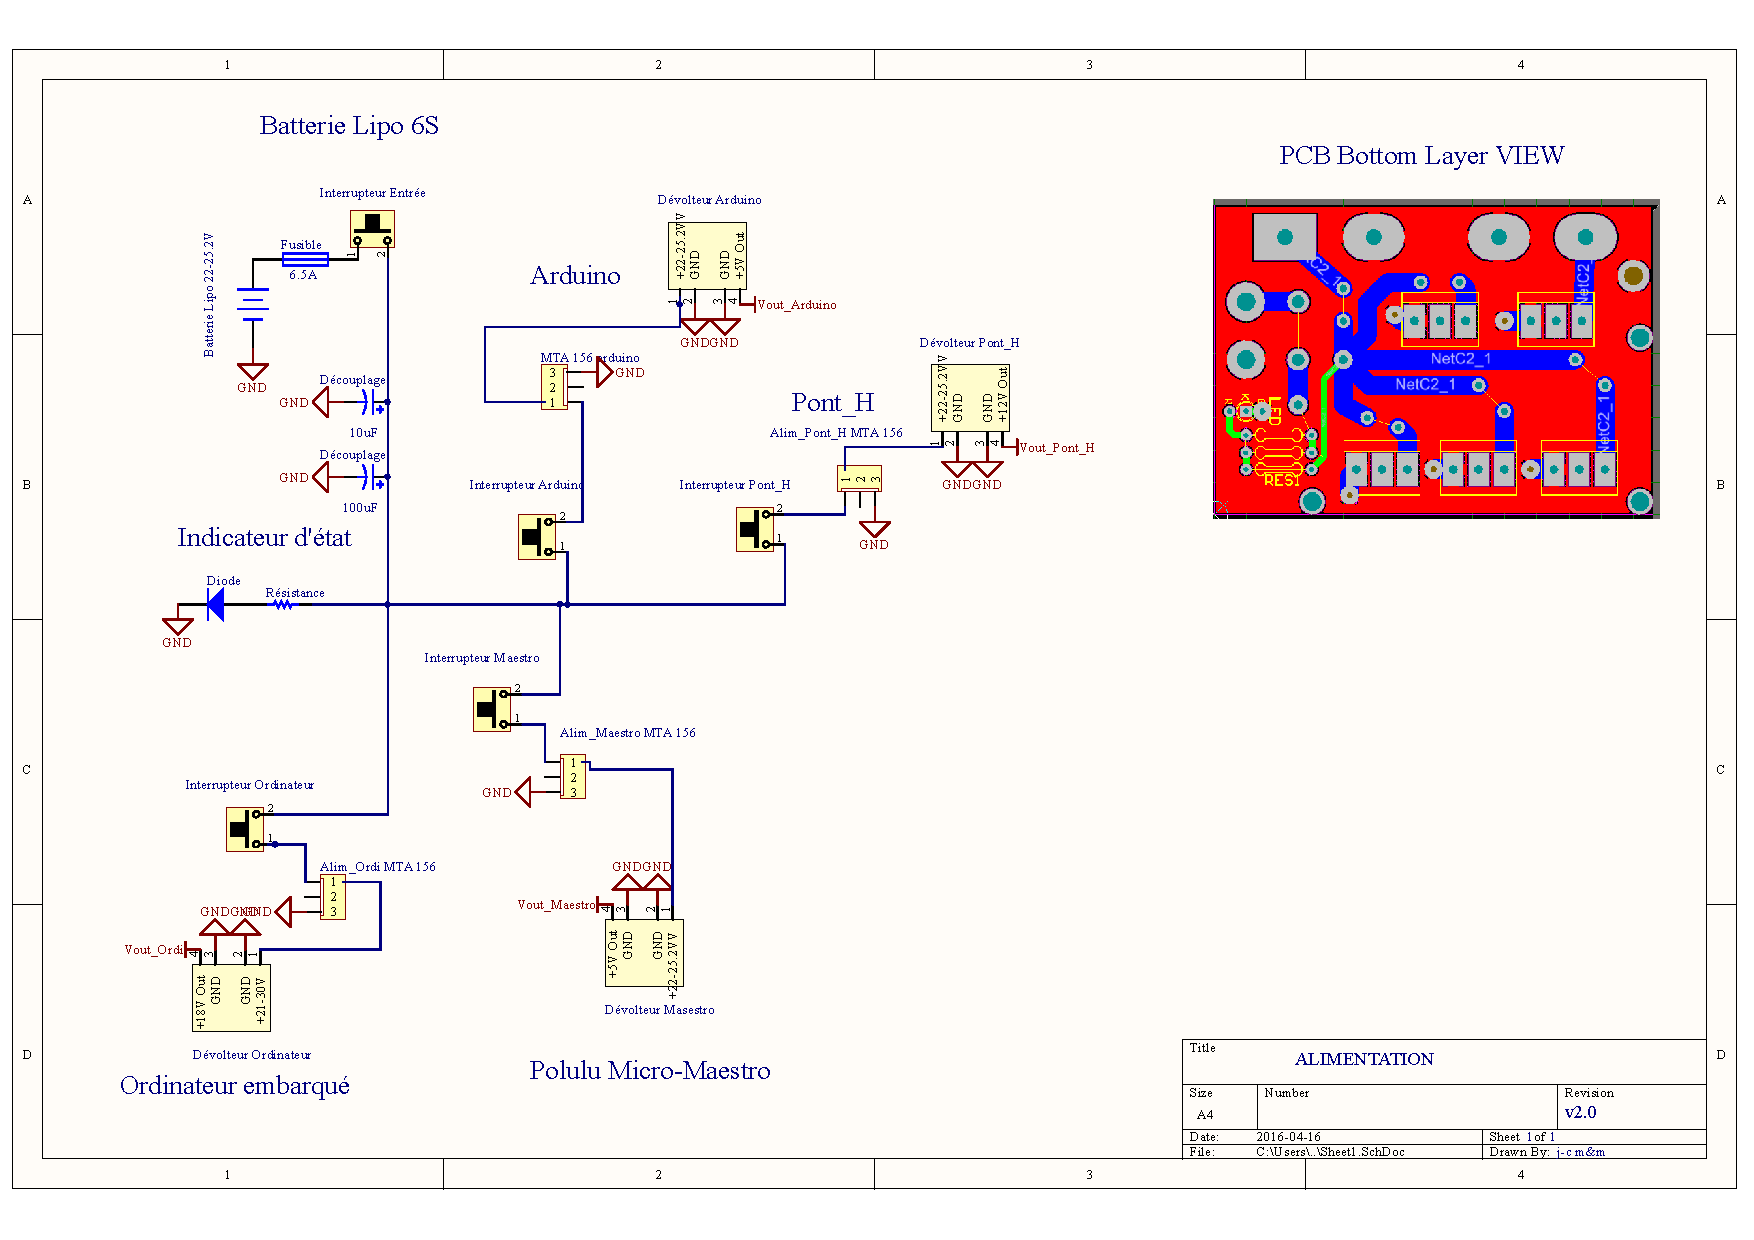
\includegraphics[scale=0.6]{resources/alim.pdf}
    \caption{Schéma électronique de l'alimentation}
    \label{fig:alim}
  \end{figure}

  \begin{figure}[ht]
    \centering
    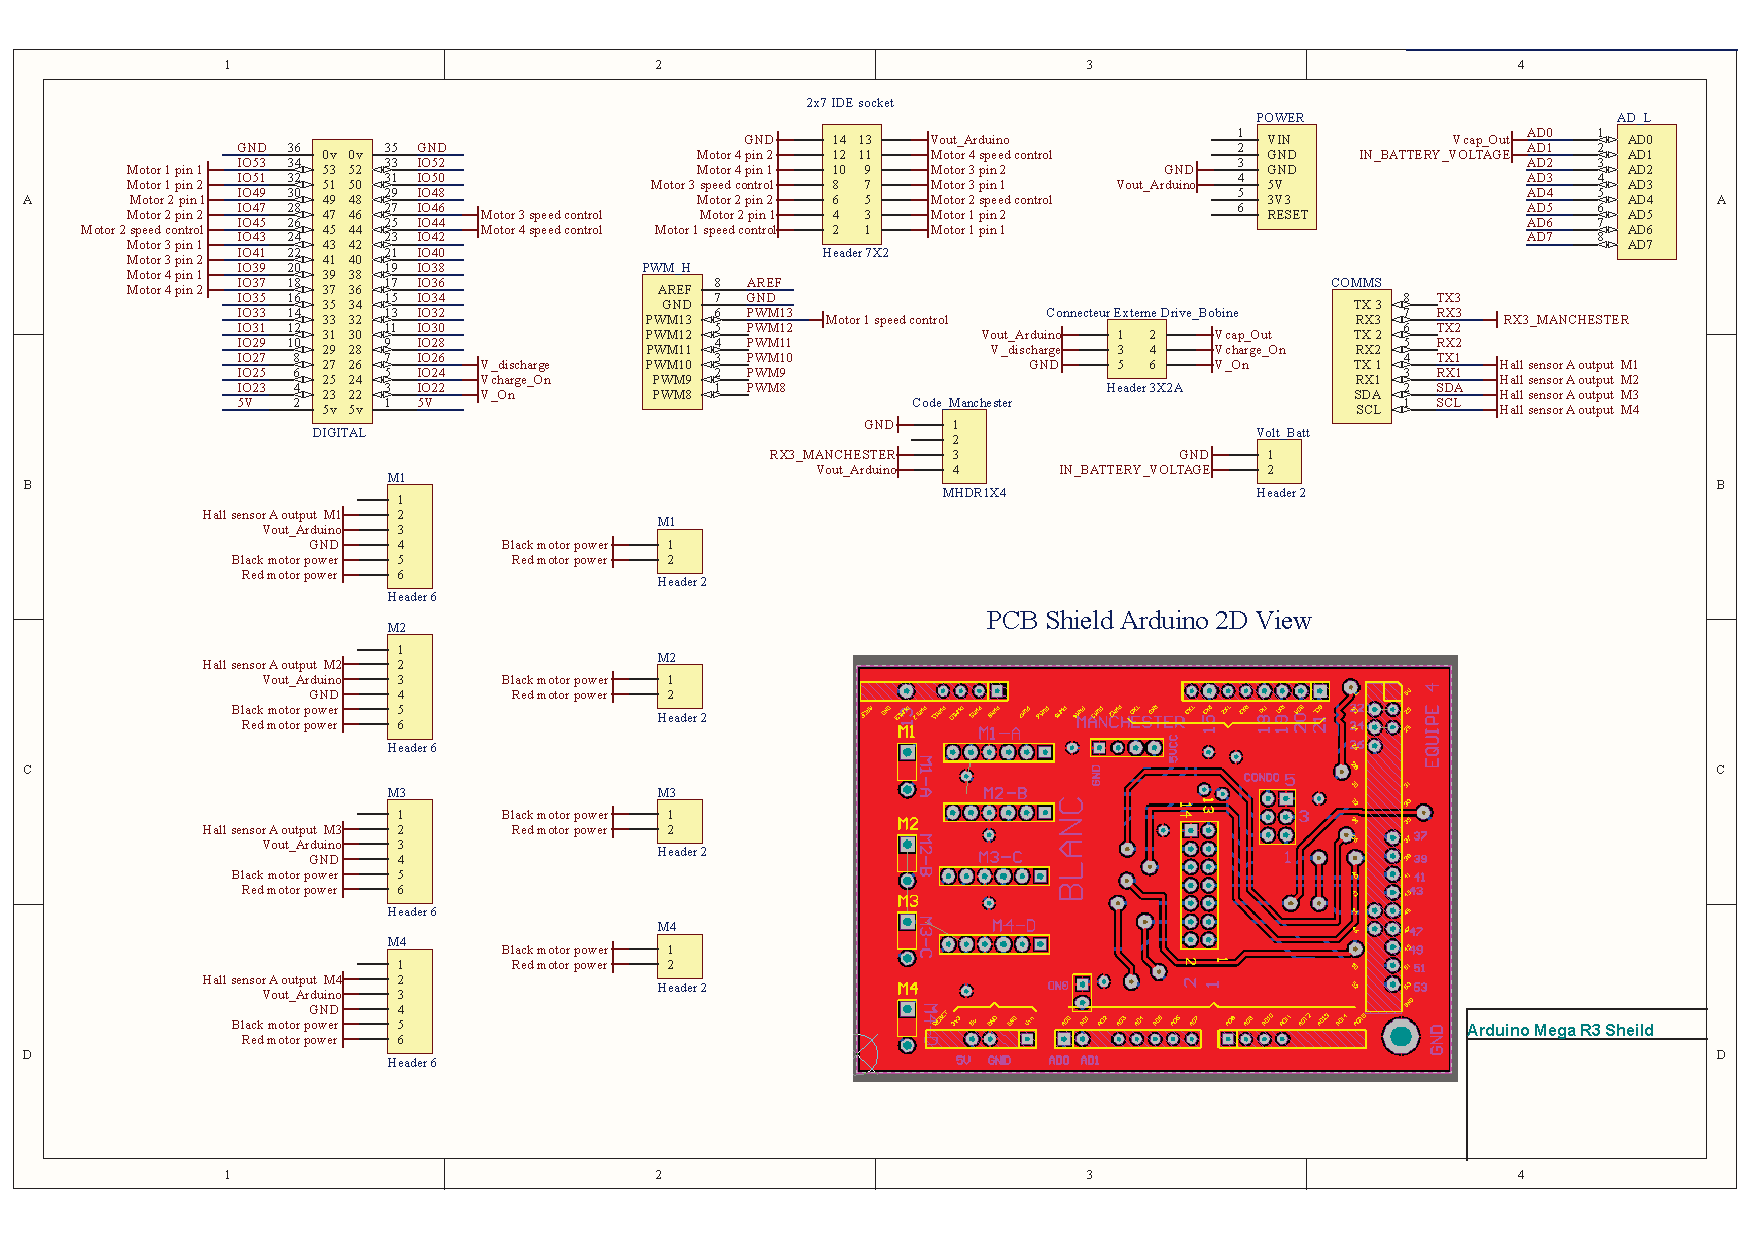
\includegraphics[scale=0.6]{resources/shield.pdf}
    \caption{Schéma électronique du shield de l'arduino}
    \label{fig:shield}
  \end{figure}
\end{landscape}

\section{Asservissement des moteurs}

L'asservissement est une partie très importante du robot, permettant de s'assurer que les déplacement des roues correspondent aux commandes envoyées peu importe les perturbations externes. Pour être fiable, une boucle de rétroaction doit être calibrée avec les bonnes constantes et doit s'éxécutée rapidement.
\paragraph{}
Afin d'asservir les mouvements du robot, chaque moteur possède une boucle de rétroaction en vitesse de type PI éxécutée à une fréquence de 20Hz. Pour connaitre la position des roues, les encodeurs à effet Hall sont utilisés. Puisque la direction des roues sont connues, un seul channel par encodeur est utilisé. À chaque front montant de l'encodeur, une interruption survient dans le microcontroleur, qui ne fait que décrémenter le nombre de \textit{ticks} restant. Ainsi, lorsque la boucle de rétroaction est éxécutée, il est possible de compter la différence de position depuis la dernière itération, et donc d'en déduire la vitesse actuelle des roues. 
\paragraph{}
Suite à plusieurs essais et expérimentations, il fut convenut que les constantes optimales pour la régulation des roues en vitesses sont $KI = 0.03$ et $KP = 0.05$. 
\paragraph{}
Parallèlement, une seconde boucle de rétroaction est utilisée pour s'assurer que le robot se déplace en ligne droite. En effet, lors des mouvements en ligne droite, les roues opposées ont toujours la même instruction. La deuxième boucle de rétroaction agit donc sur la différence des positions des roues opposées. Cette différence doit être de 0, et l'asservissement sert à ralentir une roue si elle prend de l'avance sur la roue opposée. Les constantes utilisées sur ce second asservissement sont $KI = 0.0075$ et $KP = 0.015$.
\section{Induction}

Le circuit représenté à la figure \ref{fig:induction} sert à induire un maximum de puissance au circuit de l'actionneur.
Un signal PWM est envoyé à partir du arduino de la station de base, ce dernier est amplifier par l'étage de puissance formé par les transistors.

\begin{figure}[ht]
  \centering
  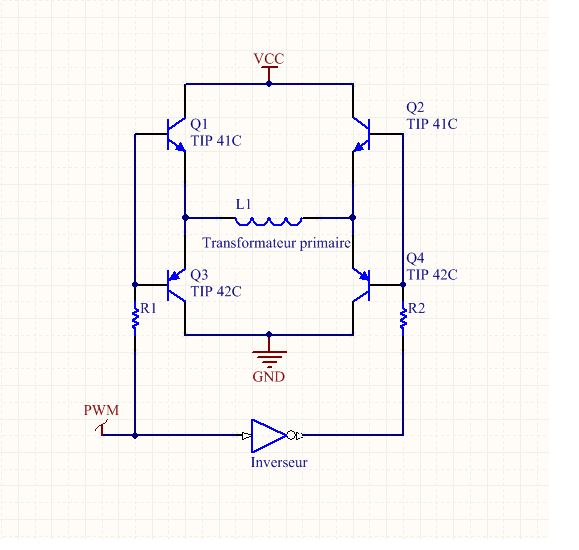
\includegraphics[scale=0.4]{resources/induction.png}
  \caption{Schéma électronique du circuit d'induction}
  \label{fig:induction}
\end{figure}

\section{Électroaimant}

\subsection{Chargeur du condensateur}

%%% Image chargeur
  \begin{figure}[ht]
    \centering
    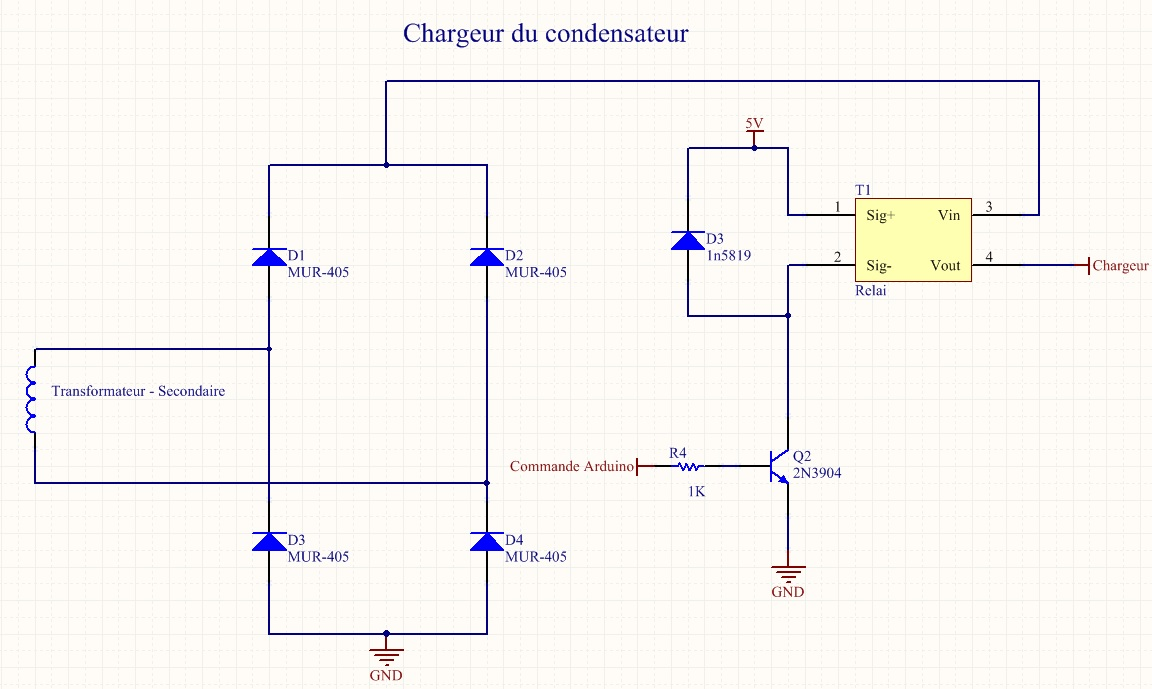
\includegraphics[scale=0.4]{resources/chargeur.jpg}
    \caption{Schéma électronique du chargeur du condensateur}
    \label{fig:chargeur}
  \end{figure}

La première étape de la charge du condensateur telle que représentée sur la figure \ref{fig:chargeur} est le redressage. On utilise un pont diodes pour redresser notre signal alternatif. Par la suite, on entre ce signal dans notre relai qui relie le pont de diodes aux condensateurs. Il s'agit de la pièce T1 sur le schéma. L'activation du relai est commandé par le arduino qui envoie un signal 0-5 volts dans la base du transistor qui \textit{drive} la bobine qui permet de fermer l'interrupteur du relai. Lorsqu'on active le relai, celui-ci devient un court-circuit et à cause que notre charge est inductive on charge à la vitesse maximale que le circuit d'induction peut fournir la puissance. En effet, si on applique une tension continu aux bornes d'un condensateur, on obtient un théorie un courant infini. Cependant, ici le courant est limité par le circuit d'induction.

\subsection{Électroaimant et voltage des condensateurs}

%%% image electroaimant_probage
  \begin{figure}[ht]
    \centering
    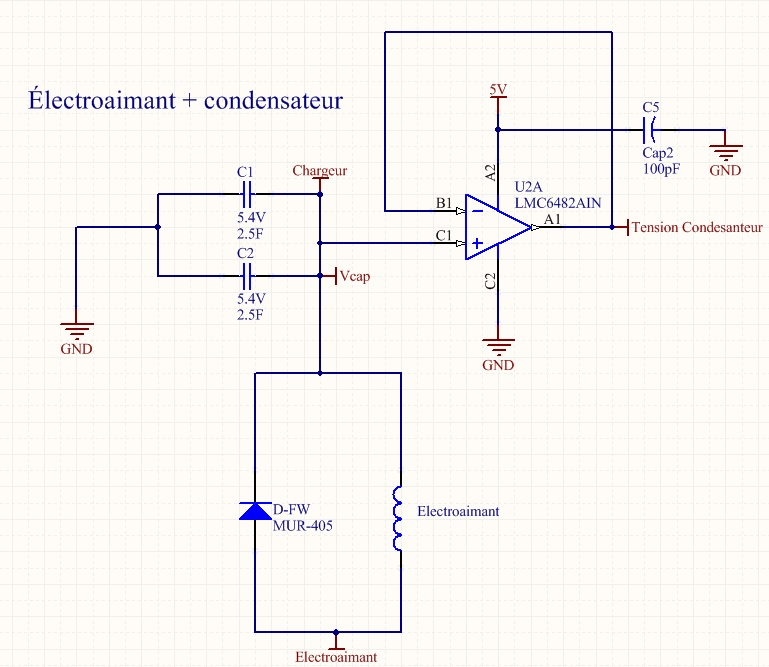
\includegraphics[scale=0.4]{resources/electroaimant_probage.jpg}
    \caption{Schéma électronique de l'électroaimant}
    \label{fig:electroaimant}
  \end{figure}
 
On observe sur la figure \ref{fig:electroaimant} la banque de condensateur qui sert à alimenter notre électroaimant. On mesure la tension des condensateurs avec un amplificateur opérationnel Rail-to-rail en mode suiveur. La sortie de cette amplificateur est fournit au convertisseur analogique-numérique du Arduino. On a mis un condensateur de découplage sur son alimentation pour limiter le bruit sur l'alimentation.

\subsection{Régulation du courant dans la bobine}

%%% image regulation_current
  \begin{figure}[ht]
    \centering
    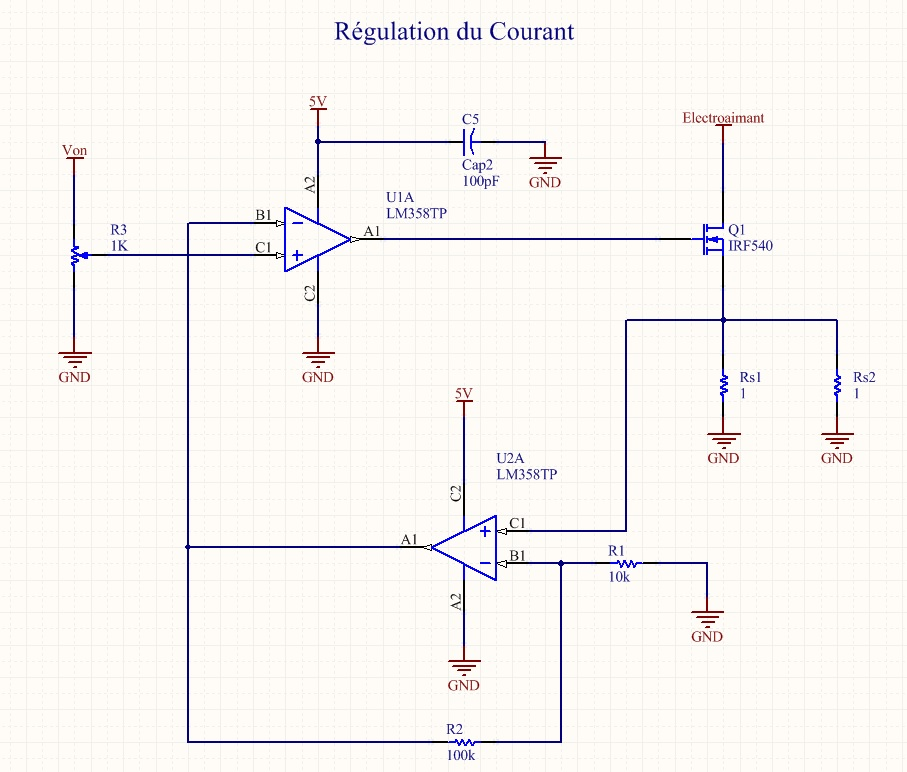
\includegraphics[scale=0.4]{resources/regulation_current.jpg}
    \caption{Schéma électronique de la régulation du courrant}
    \label{fig:reg_current}
  \end{figure}
Un régulateur analogique, tel que représenté à la figure \ref{fig:reg_current} est utilisé pour garder le courant constant dans la bobine. Pour ce faire, une source courant est créée avec un MOSFET, dont la consigne provient de l'erreur entre la commande et le courant mesuré dans le canal du MOSFET qui a été amplifié par une amplificateur en mode non-inverseur. La consigne est Von provient du arduino qui peut allumer ou fermer l'électroaimant. Encore ici, on a mis un condensateur de découplage sur l'alimentation de l'amplificateur.

\subsection{Décharge du condensateur}

%%% decharge
  \begin{figure}[ht]
    \centering
    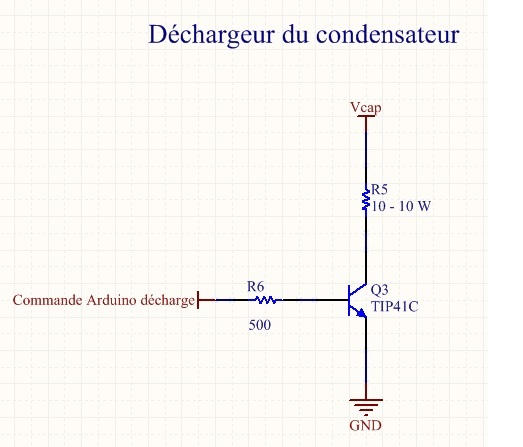
\includegraphics[scale=0.6]{resources/decharge.jpg}
    \caption{Schéma électronique de la décharge du condensateur}
    \label{fig:decharge}
  \end{figure}

Pour vider la charge dans le condensateur. On procède simplement en utilisant un transistor qui permet de vider la charge du condensateur dans une résistance de puissance, tel que sur le shéma de la figure \ref{fig:decharge}.
\section{Préhenseur}

Un préhenseur est requis afin de soulever le trésor et l'amener à destination.
Afin d'économiser la charge du condensateur, il faut miniser le temps où l'électroaimant est allumé.
Il est donc optimal de soulever le trésor à l'horizontal, dans une position où il repose sur une surface plate.

Pour ce faire, le préhenseur est constitué d'un arbre entraîné par un servo-moteur contrôllé par le pololu,
comme on peut voir sur la figure \ref{fig:lift_down}.
L'électroaimant destiné à prendre le trésor est fixé au milieu de l'arbre.
Lorsqu'un trésor est pris par le préhenseur, il est soulevé puis basculé contre un muret de bois comme sur la figure \ref{fig:lift_up}.
Il est alors possible de conserver le trésor sans qu'aucune puissance ne soit consommée.

\begin{figure}[ht]
  \centering
  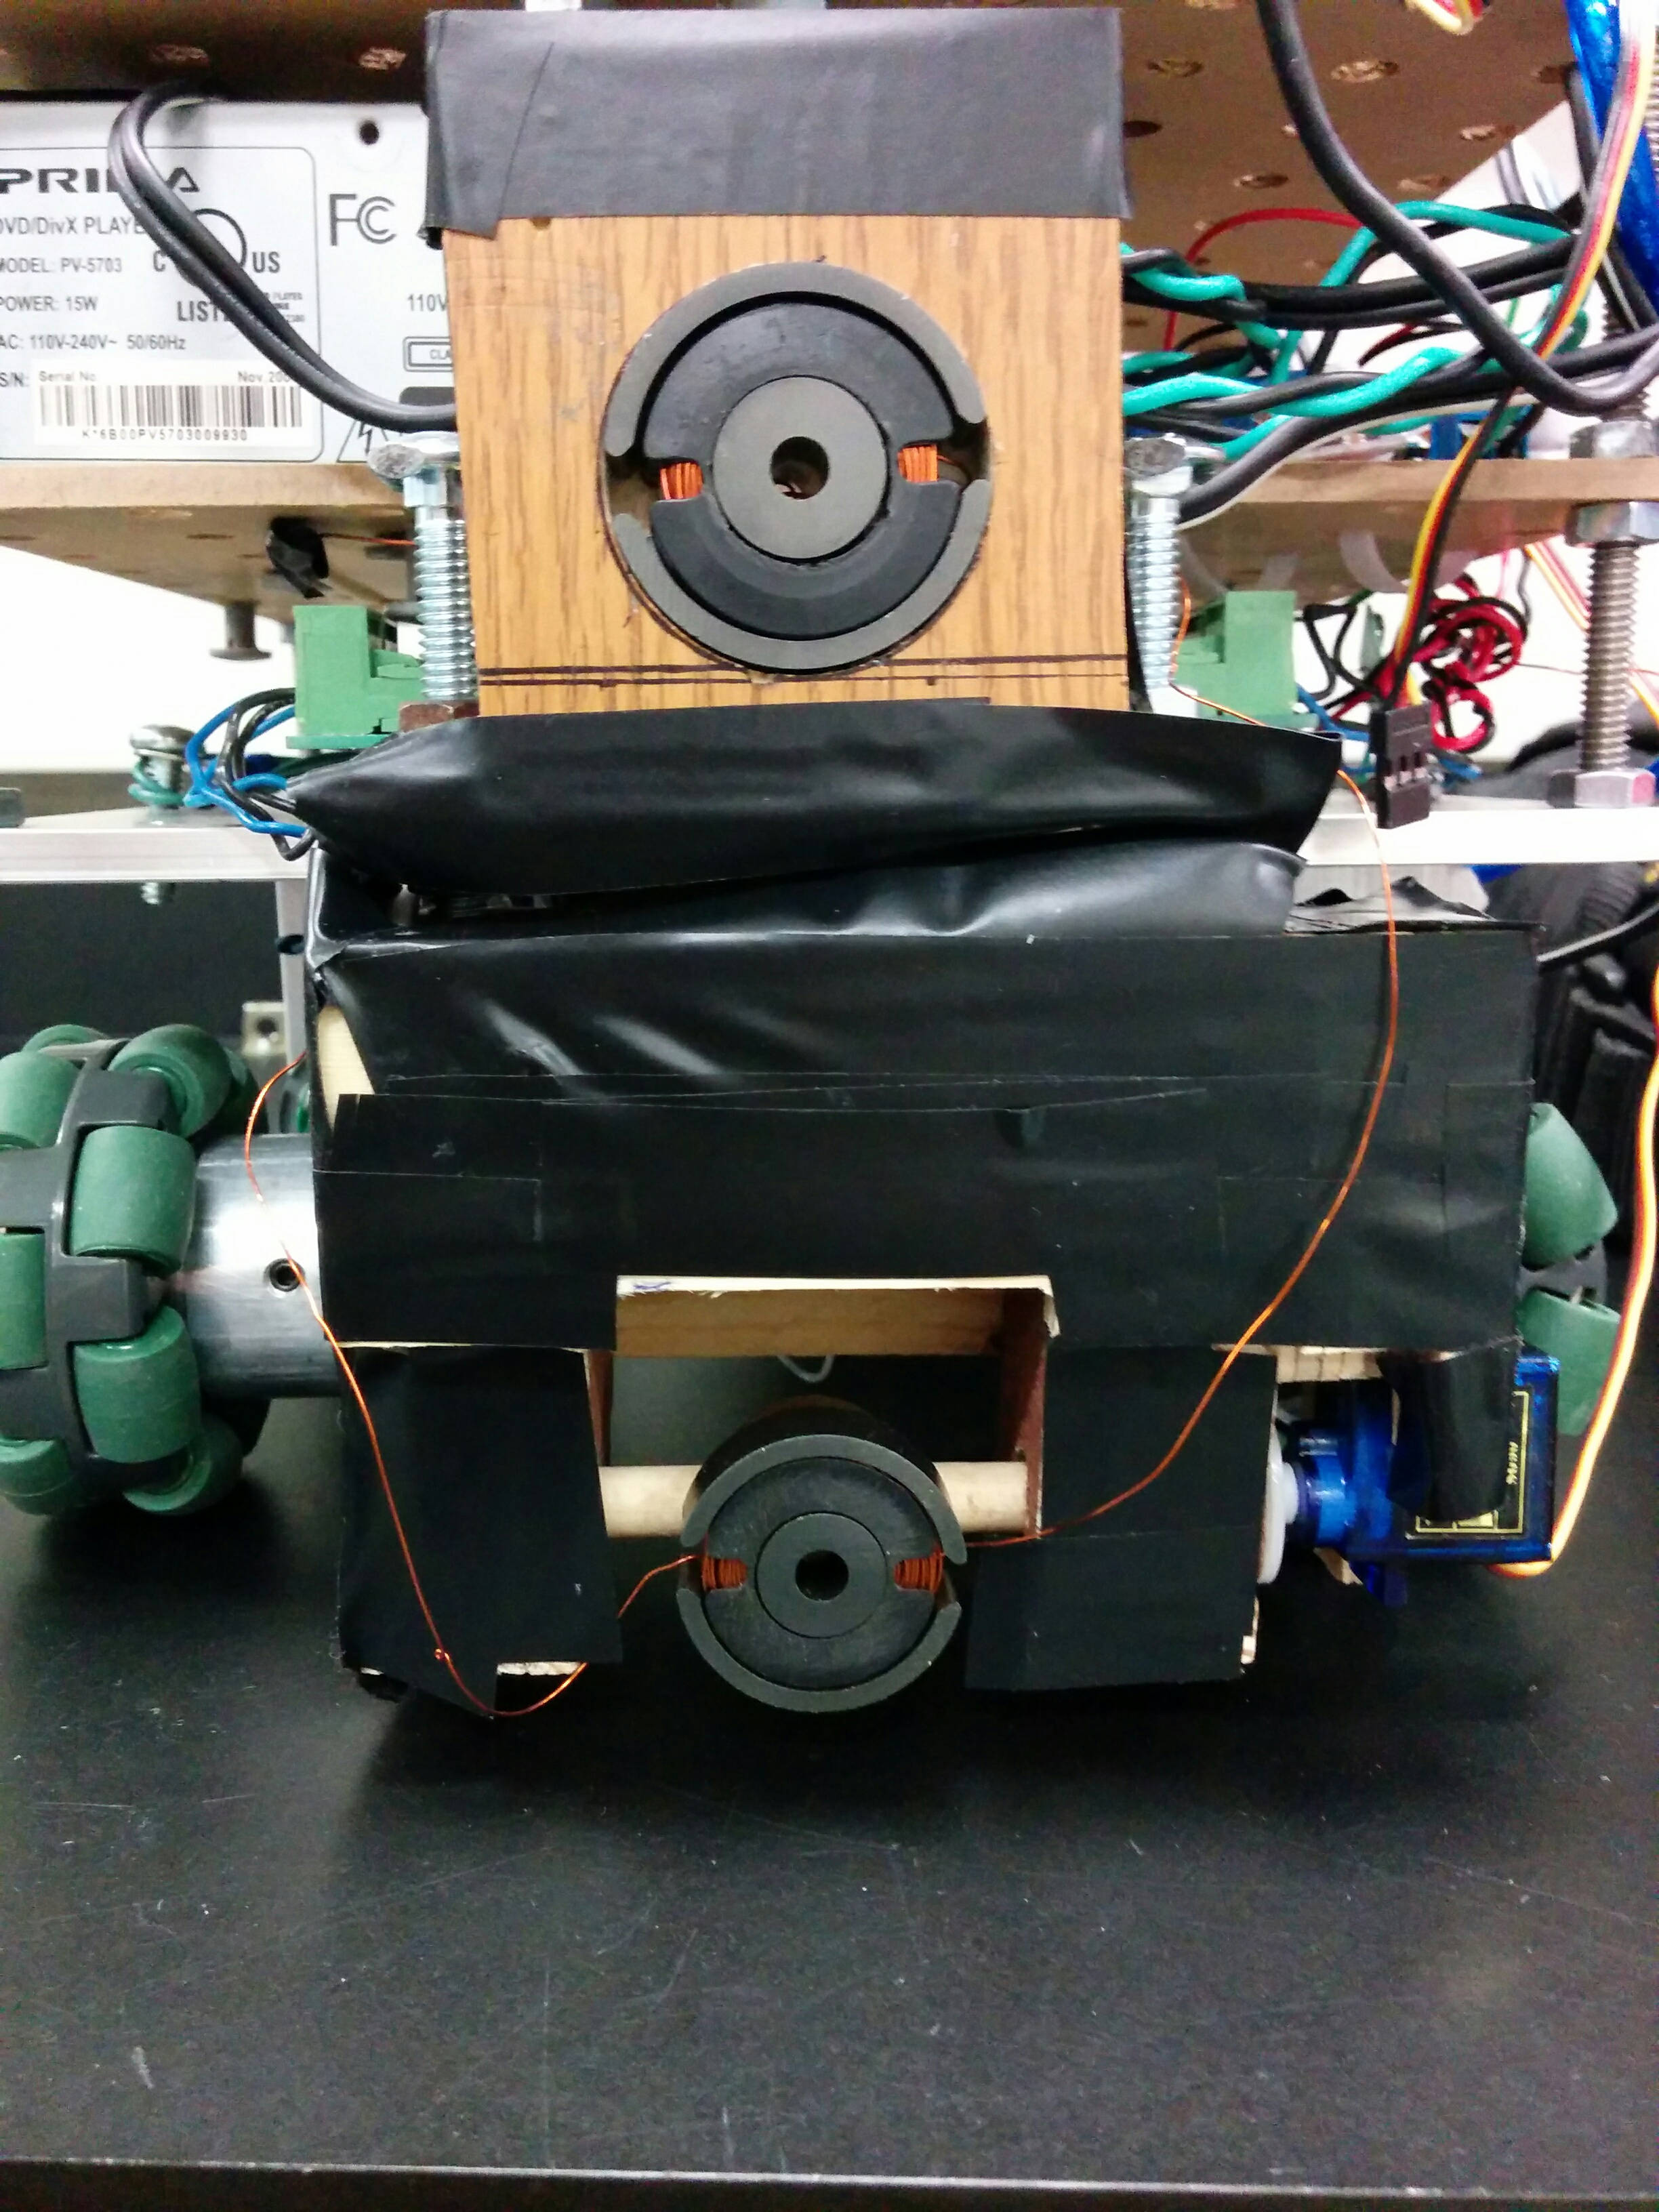
\includegraphics[scale=0.05]{resources/prehenseur_down.jpg}
  \caption{préhenseur en position de prise de trésor}
  \label{fig:lift_down}
\end{figure}

\begin{figure}[ht]
  \centering
  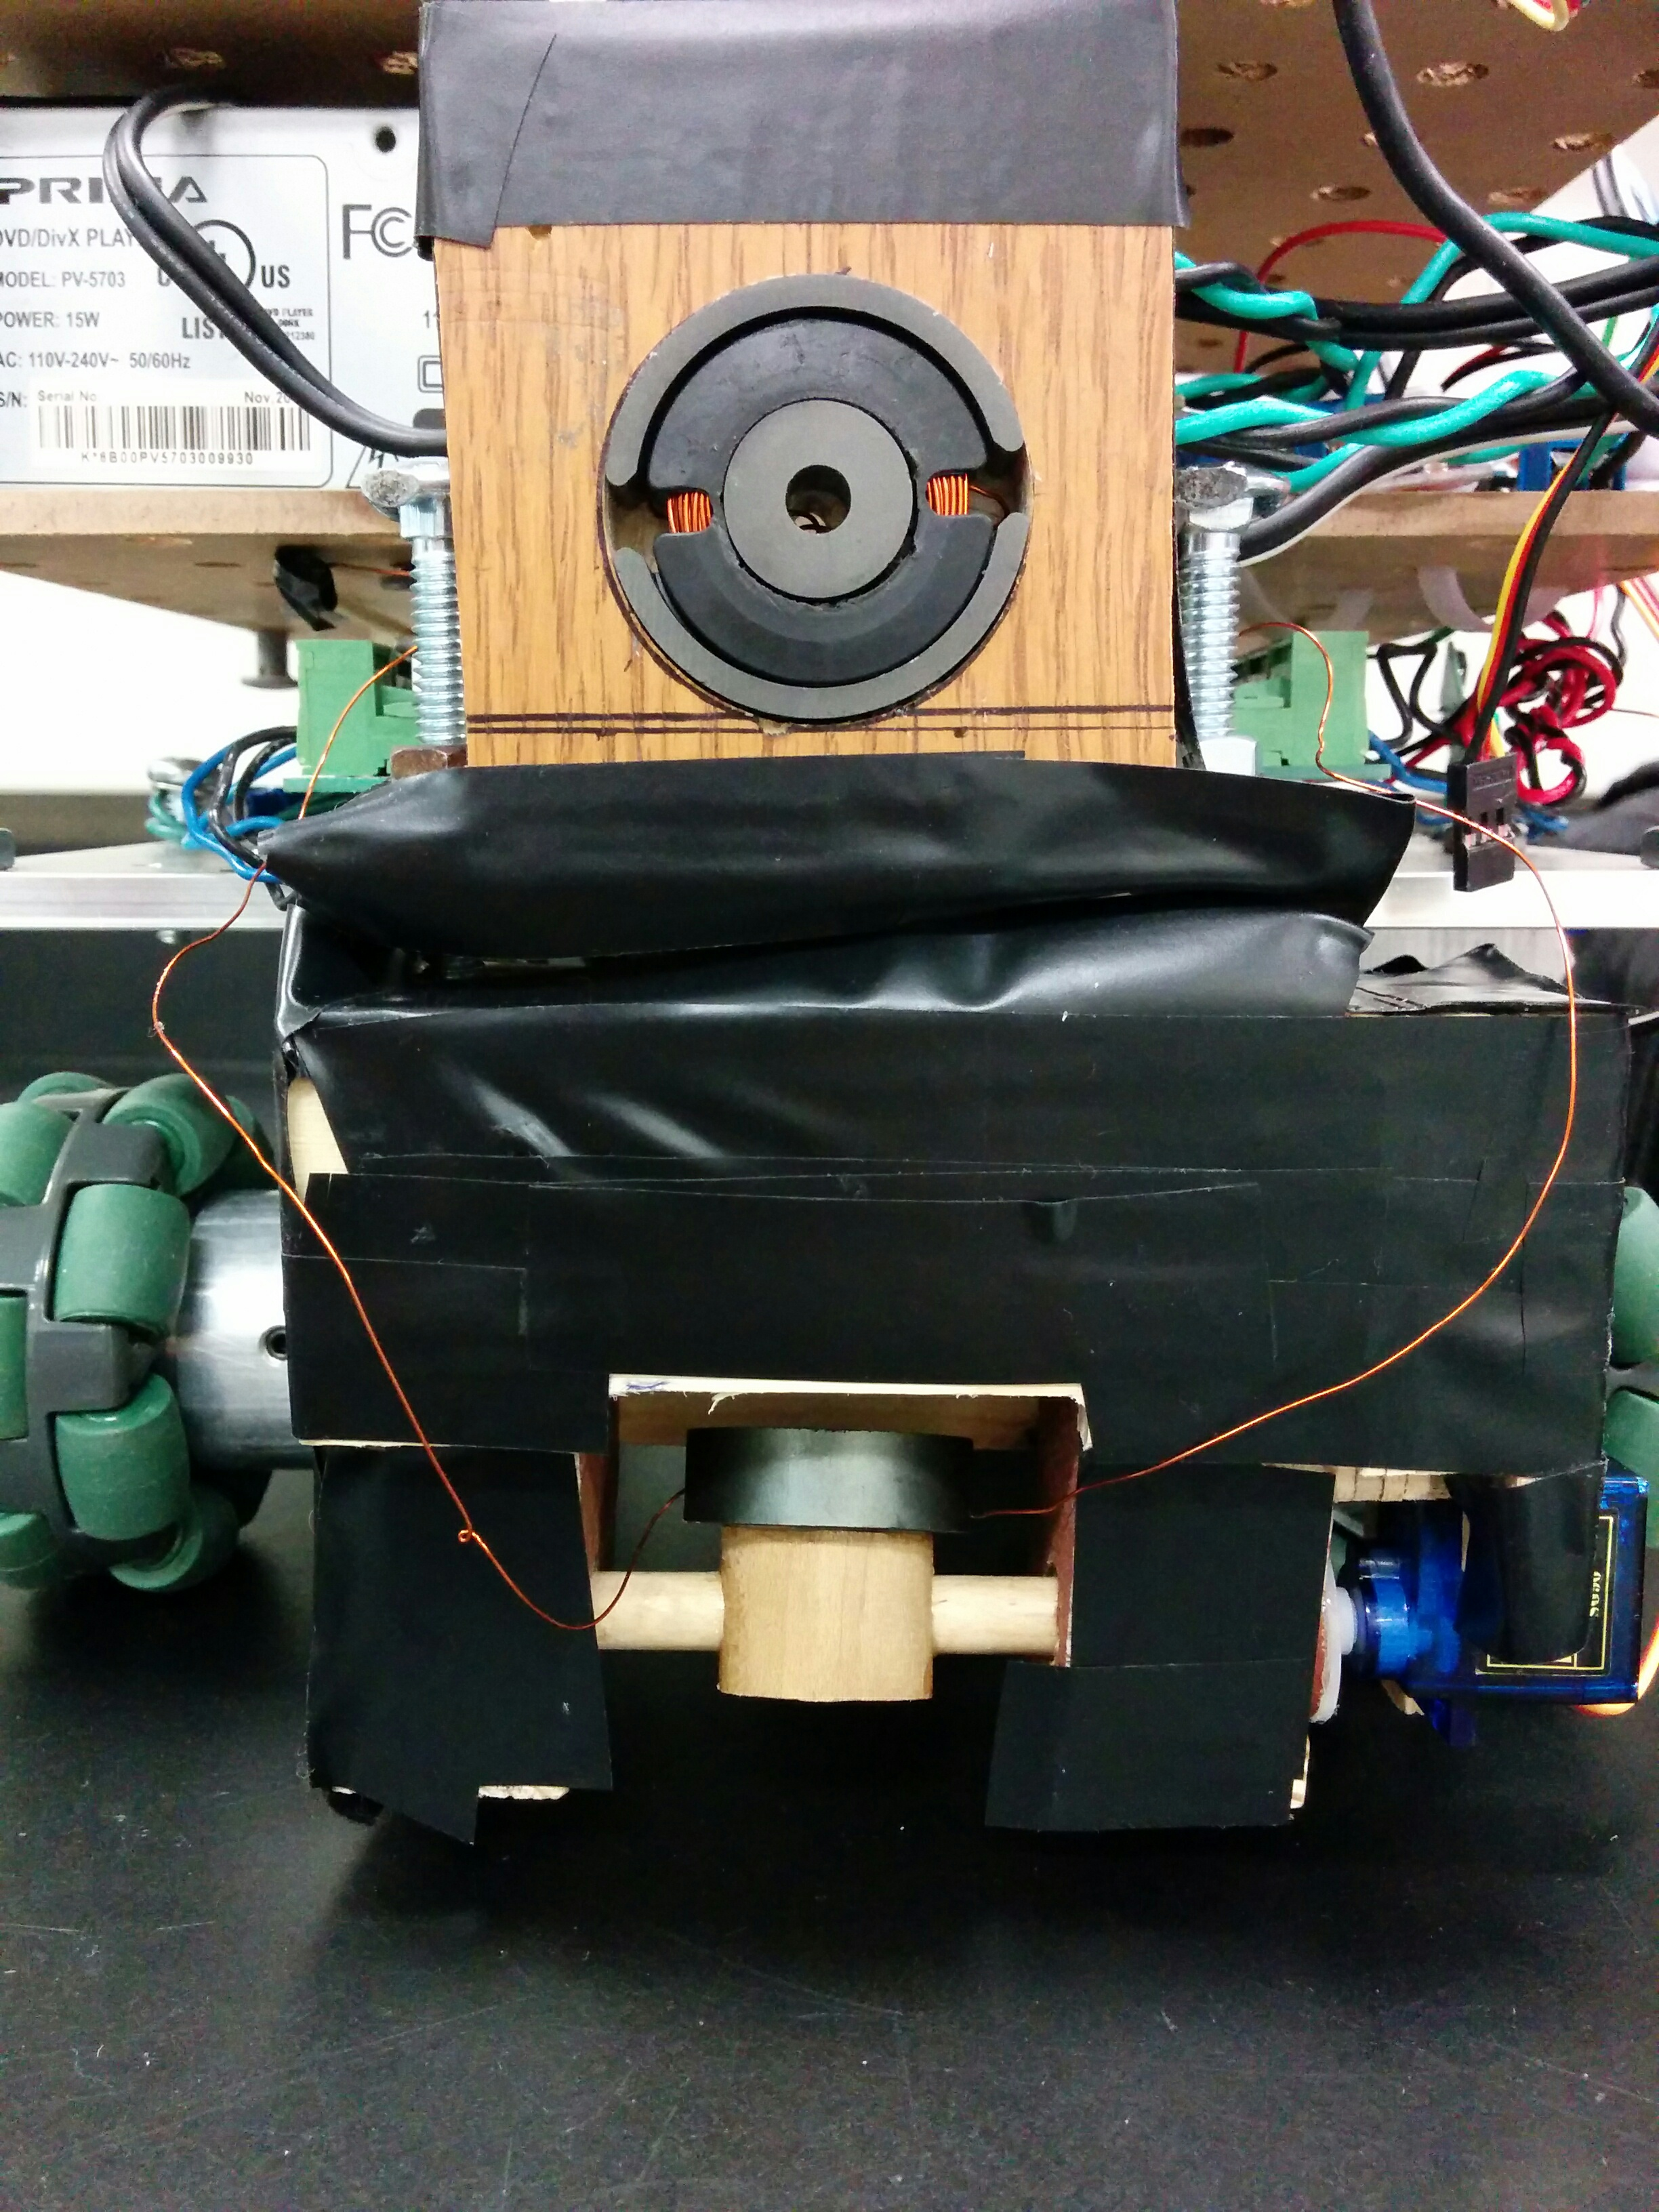
\includegraphics[scale=0.05]{resources/prehenseur_up.jpg}
  \caption{préhenseur en position de conservation du trésor}
  \label{fig:lift_up}
\end{figure}

\section{Transmission et décodage du code manschester}

Afin de transmettre le code manchester entre la station de base et le robot, un module transmetteur et un récepteur de fréquence radio 433 MHz sont utilisés.
Pour ce faire, un microcontrôleur de type Arduino Mega se trouvant à la station de base lit d'abord le code manchester en se synchronisant par interuption
sur le signal de l'horloge, sans le décoder. Par la suite, un port TX est utilisé afin de diffuser en continu le code avec un baudrate de 600 dans le transmetteur
RF. Sur le robot, le récepteur RF est branché sur un port RX avec le même baudrate que le transmetteur. Il suffit alors de lire le contenu du buffer
série 4 fois (4x8 bits) afin d'obtenir les 32 bits du code manchester qui est décodé par la suite sur le Arduino. Le Arduino décode continuellement le
contenu du buffer série.
\paragraph{}
Puisque le signal d'horloge n'est pas transmis, il faut trouver le point de départ en identifiant la séquence de 18 bits fixes de départ
(le signal de données manschester contient deux fois plus de bits que le code original). Une fois cette séquence de départ identifiée,
il suffit de décoder les 14 bits restants. Pour ce faire, les bits sont simplement regroupés en sous-séquences de deux bits.
Une sous-séquence 0-1 signifie un '1' tandis qu'une sous-séquence 1-0 signifie un 0. Tout autre sous-séquence est interprétée comme une erreur et on recommence
l'acquisition du code manchester. Suite à ce décodage, une séquence de 7 bits est obtenue, correspondant au signal ASCII désiré. Si le contenu ne correspond
pas à un code manchester (même nombre de 1 que de 0, 8 bits à "1" de suite suivi d'un bit à "0"), le dernier code manchester valide est
gardé en mémoire jusqu'à ce qu'un autre code valide le remplace. L'ordinateur embarqué peut en tout temps demander le dernier code manchester décodé valide.

\chapter{Bilan post-mortem}
 
Lors d'un projet d'envergure comme celui de Design 3, il est important d'y jeter un regard en rétrospective et d'en retirer des leçons. Par exemple, déterminer les points forts et les points faibles permet de réfléchir sur les choix de design effectués au cours de la session et de s'améliorer en tant qu'ingénieur.
\section{Points forts du robot}

Analyser les points forts du projet permet de conserver les bons choix de design pour les projets futurs. Cela permet aussi de s'encourager et de regarder le projet avec fierté.

\subsection{Vision World}

La vision de la caméra world était très solide. En effet, un masque était d’abord construit de façon à couper l’image autour de la surface de jeu de façon à limiter l'environnement où détecter les îles et les trésors. Les coins de la table étaient trouvés grâce au carré vert de calibration au centre de la table. Les algorithmes de détection des îles et des trésors avaient des filtres de couleurs larges afin de pouvoir s’adapter à plusieurs situation lumineuses différentes. Pour ensuite différencier les îles où les trésors du bruits ou de d’autres objets aux couleurs similaires, des filtres de dimensions, de formes et de positions précis pouvaient être utilisés en raison du fait que la caméra était statique. Le résultat était une détection parfaite de tous les éléments à tous les coups.

\subsection{Asservissement des moteurs}
L'asservissement des moteurs nous a permi de faire tous les mouvements nécéssaires avec une grande précision. Les mouvements étaient entièrement omnidirectionels et indépendants de l’angle du robot. Six boucles PID furent utilisées sur le microcontroleur: Une indépendante pour chaque moteur, en vitesse, et une par paire de roues ayant la même orientation, en position. La première boucle en vitesse était très rapide et permettaient d’aller a des vitesses élevées sans dépassement. La deuxième faisait toute la magie: en comparant la position des roues opposés, la boucle assurait que les roues étaients toujours au même point dans leur commande respective, et donc garantit un mouvement en ligne droite. Lorsqu’une roue est bloquée pendant un instant, elle est accélérée afin de surmonter l’obstacle tandis que l’autre est freinée. Lorsqu’une roue se met à glisser et accélère subitement, elle est freinée par l’état de l’autre roue. Lorsqu’il y a un désiquilibre de poids sur le robot causant l’accélération d’une roue, la boucle compense cette différence.

\subsection{Préhenseur et système de recharge}
Le préhenseur construit est certainement un point fort du robot. Une base en bois lui offre une structure solide qui permet de se coller sur le trésor sans s’abimer. Il peut également effectuer une rotation afin de garder le trésor dans une position de rétention permettant d’économiser de l’énergie. Ce choix de design a sauvé beaucoup de temps sur la conception du système d’électroaimant, puisque la rotation du préhenseur permet une prise de trésor peu couteuse en énergie.

De plus, le système d’alimentation de la bobine est construit avec un asservissement analogique, donc le microcontroleur n’a qu’à envoyer un 5V pour l’activer et un 0V pour l’éteindre. Ce système était une excellente décision, réduisant la logique du microcontroleur et le traitement nécéssaire pour activer le préhenseur. C’est également le cas pour l’activation de la recharge du condensateur, interfacé avec une commande 0-5V.

D’ailleurs, la séquence de dépot du trésor active l’électroaimant avant de descendre le trésor, permettant de garder un controle absolu sur le trésor.

Finalement, la structure du préhenseur et de la bobine d’induction est construite avec un ressort, permettant au robot d’épouser l’angle du mur du trésor et de la station de recharge lors du contact.

\subsection{Alignement à l'aide de la vision embarquée}
Le système d’alignement du robot avec les trésors et la station de recharge est très rapide. L’excellent asservissement de la position du robot et la vision world précise permettent d’abord de positionner le robot à un endroit très près du trésor, dans le bon angle. À cet instant, seul un petit ajustement latéral est requis, ce qui est accompli avec la caméra embarqué. Il ne suffit que d’identifier et de “track” la cible (à plus de 30 images/seconde) et de se déplacer dans la bonne direction (gauche ou droite) avec une répétition rapide (5 Hz) de petits mouvements  (mouvement minimum des roues) jusqu’à ce que le robot soit enligné avec la cible. Cette séquence a permis à notre robot de s'aligner très précisément (2-3 mm) dans un intervalle de temps très petit (4-5 secondes).

\subsection{Robustesse aux pertes de connexion}
La séquence complète de jeu a été divisée en plusieurs actions, qui pouvaient alors être chainées afin d'accomplir un tour du jeu. Ceci nous permettait de vérifier lors des étapes cruciales que le robot possédait bien une connection Wi-Fi. Lorsque cela se produisait, nous stoppions aussi tout mouvement puisqu'une boucle de rétroaction impliquant le Wi-Fi est nécessaire pour obtenir un bon déplacement.

\subsection{Simulation logicielle du robot}
Nous avons programmé une simulation logicielle de la plupart des actions du robot telles que le déplacement suivant le chemin trouvé. La simulation était intégrée avec la vision de la caméra world qui était reproduite à partir d’images de la table. Il donc possible de voir le robot simulé se déplacer en évitant les îles détectées par la vision dans l’interface web. Cette simulation nous a permis de voir les effet de notre code tôt dans le projet et de corriger plusieurs erreurs, qui, autrement ne seraient apparus que lors de l’intégration avec les composantes matérielles.

\subsection{Alimentation}
La présence d’interrupteur pour chaque composante permettait de faire la sélection en alimentation des composantes seulement sollicitées lors des bancs de test. De plus, lorsque l’ensemble des composantes était alimenté par la batterie, le robot était fonctionnel jusqu’à 3h consécutif. Ce temps d’utilisation est en lien direct avec le choix d’une batterie de 5200mAh. Un fusible d’entrée s’est avéré utile, et lors d’un mauvais branchement d’un dévolteur, nous avons constaté l’importance de sa présence sur le circuit d’alimentation.
\section{Améliorations potentielles du robot}

Réaliser que le produit final n'est pas parfait est une étape importante dans le processus de design si l'on souhaite observer une amélioration. Le robot était loin d'être parfait, et plusieurs améliorations possibles auraient pu être faites si plus de temps était fourni.

\subsection{Disposition physique du microcontrolleur}
Ne pas fixer le arduino sous le robot en ayant comme seul isolant le plastique de l’emballage du arduino. En effet, il n’aurait suffit que d’un mince trou dans le plastique pour court-circuité le microcontroleur.

\subsection{Callback du Arduino à la fin d’une commande complétée}
En ajoutant un \textit{callback} à la fin d’un mouvement du Arduino, le programme n’aurait pas eu besoin de renvoyer la commande de mouvement à toutes les 250 ms. Le programme pourrait alors laisser le Arduino travailler et terminer sa commande. Cela éviterait de renvoyer une commande pendant un déplacement, qui en raison du délais de la vision, créait un dépassement de la commande à tout coup puisque la position détectée et la position réelle étaient différentes.

\subsection{Estimation de la position à partir des encodeurs}
En estimant la position du robot à partir des encodeurs, le robot aurait pu être autonome même quand la caméra world ne pouvait plus le détecter. Ce mode de fonctionnement aurait permis au robot d’aller facilement au fond de la table sans perdre le contrôle sur sa position.

\subsection{Vision des trésors du fond}
Avoir eut plus de temps nous aurions terminé l'intégration de la gestion des trésors du fond qui sont hors de portée de la caméra world. En effet nous pouvions les détecter et les ajouter à notre "worldmap", mais nous n'avions pas un système de déplacement assez robuste alors nous avons préféré ne pas les prendre en compte.
Ce qui nous amène au point que nous aurions voulu améliorer le déplacement du robot dans des zones sans vision du dessus.

\subsection{Système de traitement des erreurs dans le séquenceur}
Nous aurions aimé avoir le temps d’ajouter de la robustesse au séquenceur des actions du robot. Par exemple, si le robot échappe le trésor, il aurait été possible de le détecter avec la caméra embarquée et de recommencer l’action. De la même façon, si aucun chemin n’est trouvé par le robot pour se rendre au trésor ciblé ou à l’île cible, la vision ou le manchester auraient pu être rafraîchis et l’algorithme recommencé. 

\subsection{Logger}
Au cours du développement nous avons enlevé la composante "logger" du système afin d'enlever de la complexité, mais finalement celui-ci se serait avéré assez utile. Surtout lors des derniers tests lorsque le robot est tout intégré et que nous ne voulons pas avoir à l'ouvrir pour savoir ce qui se passe.

\subsection{Interface}
Nous aurions aussi aimé améliorer l'interface en ajoutant plus d'information, tout en améliorant son accessibilité. Par exemple nous aurions ajouté l'information sur le niveau de charge de la batterie et un "feedback" dans la section de lancement des différentes séquences.

\subsection{Alimentation}
Il aurait été préférable d’avoir un fusible pour chacune des composantes du robot. Une meilleure préparation en vue de l’assemblage du robot aurait permis de constater que la longueur des fils utilisés était inutilement trop grande pour les divers interrupteurs. Aussi, il aurait été plus sage de mettre un plus grand nombre de condensateurs de découplage. 

\section{Retour sur les choix de design (Si le projet était à refaire...)}

Maintenant que le projet est terminé, plusieurs choix sont regrettés. Il est essentiel de regarder le projet avec du recul et de se demander qu'est-ce qui aurait pu être changé dès le début du projet pour faciliter la tâche. Ainsi, si le projet était à refaire du début, certaines choses seraient faites autrement.

\subsection{Revoir le choix du langage de programmation}
Puisque le python n’est pas un langage typé, nous avons passé beaucoup de temps à régler des erreurs de types. Aussi, à la fin notre programme était assez gros et plusieurs classes étaient injectées, donc l’autocomplétion n’était pas possible, ce qui a aggravé le problème. Par conséquent, si c’était a refaire, nous considérerions les langages typés dans le choix du langage même si le python nous a avantagé dans la rapidité de développement de l’architecture réseau et par sa facilité d’utilisation avec OpenCV.

\subsection{Tests fonctionnels}
Les tests fonctionnels avec tout le système intégré sont absolument essentiels pour ce type de projet. Nous en avons bien sûr fait mais pas suffisamment. Des tests plus long, s'étirant sur une semaine par exemple, nous auraient permis de d'essayer toutes les configurations possibles et de corriger la plupart des problèmes et faiblesses de notre robot, tout en nous assurant des bonnes nuit de sommeil. Bien sûr afin d'y arriver, il faut s'assurer de contrôler toute "feature envy"

\subsection{Alimentation}
Obtenir les dévolteurs le plus tôt possible. Le délai d’attente que nous avons eu pour la réception de ceux-ci et la contrainte de temps pour mettre en marche le robot nous a forcés à fabriquer le PCB de l’alimentation sans la présence de dévolteurs, outre celui de l'ordinateur embarqué. Avec une réception hâtive des dévolteurs. Nous aurions pu incorporer l’ensemble des dévolteurs au PCB de l’alimentation. Ceci aurait éliminé ainsi un grand nombre de fils. De plus, le détecteur au DEL de basse tension de la batterie manquait de précision. Si c’était à refaire, nous commanderions un indicateur de basse tension avec affiche de la tension de la batterie. 


\end{document}
